\documentclass[10pt,letterpaper]{article}
\usepackage[margin=0.85in]{geometry}
\usepackage{amsmath,amssymb,booktabs,graphicx,tabularx,array}
\usepackage[numbers,sort&compress]{natbib}
\usepackage{xurl}
\usepackage[hidelinks]{hyperref}
\title{Beyond Recall: Delivery Replay and Evidence Drift in Long-Term Memory for LLM Agents}
\author{Aditya Mantri\thanks{Independent research. Author background supplied by the author: AI Engineer at Genies; M.S. in Engineering, Purdue University. This work uses no employer code, data, credentials, or services; no employer endorsement is implied.}\\\textit{Independent Researcher}}
\date{October 30, 2026}
\begin{document}
\maketitle

\begin{abstract}
Persistent memory is commonly evaluated by asking whether a system can answer later questions. That outcome can conceal a systems failure: a write may be durably preserved, yet a repeated delivery can alter which evidence reaches the reader. We report a bounded, frozen-input development study of controlled post-effect delivery replay in two local raw-document memory paths, using 24 questions from public LoCoMo and LongMemEval development histories. Across 308 native processes, 84 injected post-effect acknowledgement cuts, and 14,320 original backend events, repeated deliveries increased physical multiplicity while preserving original point identities and source content. In one directly inspectable LongMemEval case, the latest dated recipe count remained stored and appeared at native rank 11, but was displaced from a ten-record context: both GPT-6.1-Sol repeats and a local Qwen3 reader changed from the official answer, three, to the older count, two. This is a trace-level witness, not a population rate. Retrieval-time event deduplication restored every task label flagged as a loss in this finite pilot, but did not generally restore hybrid retrieval order. In a separately specified post-hoc mechanism probe, duplicate points remained searchable while the pinned Qdrant IDF corpus was restricted to clean physical IDs; this restored all 24 Mem0 contexts and five score components within tolerance. Duplicate-induced IDF drift is established information-retrieval behavior, not our novelty claim. The candidate contribution is an auditable native replay-to-retrieval-to-reader conformance trace that distinguishes physical preservation, evidence selection, and answer outcome. The study is exploratory: its questions share source histories, automated current-conflict calibration failed, one judge is same-family as a reader, and the ranking probe reuses the same questions. It provides no external replication, population estimate, or journal-readiness claim.
\end{abstract}

\noindent\textbf{Keywords:} long-term memory; LLM agents; retrieval; duplicate evidence; retry; idempotency; reproducibility

\section{Introduction}
An agent may retain every stored record and still lose the evidence needed to answer a later question. This possibility matters because memory evaluation spans several contracts that are often collapsed into a final answer: whether a write occurred, whether a retry duplicated its representation, which records a retriever selected, and whether a reader answered from those records. Benchmarks such as LongMemEval and LoCoMo make long-horizon question answering measurable, while persistent-memory systems and architectures add storage and retrieval components to the pipeline \citep{wu2024longmemeval,maharana2024evaluating,packer2023memgpt,chhikara2025mem,xu2025amem,rasmussen2025zep}.

We examine a narrow operational question: after a storage effect has happened but before its logical acknowledgement is recorded, what can repeated delivery do to later evidence selection? The fault schedule models a worker exiting after the native write effect and before a study-level acknowledgement. The retry then repeats the same source occurrence. This is not a network packet-loss experiment, a crash in the middle of a database commit, or a natural production failure-rate measurement. It is a controlled conformance probe at a declared boundary. Reliable-effect systems have long addressed retry ambiguity through durable identity, completion records, and replay protocols; we use that literature to define the boundary rather than claim a new transaction method \citep{lee2015implementing,zhang2020fault,birrell1984implementing,fielding2022http}.

The study's clearest witness is one dated LongMemEval question about the number of Emma's recipes tried. The history says two on May 29 and three on May 30. After replay, both statements remain physically present, but duplicated older events occupy six of ten context slots and the newer count moves from native rank 5 to rank 11. Two GPT-6.1-Sol requests and one local Qwen3 request change from three to two. The trace makes the failure inspectable: there is no need to infer deletion or hallucination when the later source event is simply absent from the delivered context. It is selected from an exploratory pilot and is not a held-out test or independent peer assessment.

The result has two levels. In task-space, retrieval-time source-event deduplication recovers all automated task labels flagged as replay-associated losses in this finite pilot. In mechanism-space, deduplication alone does not recreate the original physical corpus statistics. For the local Mem0/Qdrant path, a post-hoc diagnostic that leaves duplicate points searchable but computes IDF over the clean physical IDs restores the clean full-pool contexts for all 24 questions. The latter uses oracle knowledge of the clean corpus and is not a deployable repair. These observations separate a useful simple mitigation from an explanation of residual ranking drift.

We make three bounded contributions. First, we define an observation model that separates source occurrences, physical storage instances, selected evidence, and task outcomes. Second, we provide a traceable native-store experiment with explicit post-effect acknowledgement cuts, reader inputs, response aliases, grading records, and independent audits. Third, we localize one source of residual hybrid-ranking change with a clean-statistics counterfactual, while connecting it to established work on duplicate documents and IDF rather than presenting it as a new retrieval principle \citep{frieder2003scalable,robertson2009probabilistic,schelpe2026byte,jain2026cuer,ross2026redundancy,cho2026rare}.

This is a development study, not a Q1-ready validation. Its scope is two locally instantiated raw-document APIs, 24 questions from overlapping public histories, a controlled replay schedule, and automated grading with a failed auxiliary calibration. A broader study would require held-out histories, additional native systems and model families, independent human adjudication, naturalistic failure mechanisms, and external replication.

\section{Related Work}
\subsection{Persistent memory and lifecycle evaluation}
Long-term memory research has developed architectures for explicit memory management, retrieval, reflection, and temporally structured knowledge \citep{packer2023memgpt,zhong2023memorybank,xu2025amem,rasmussen2025zep,latimer2025hindsight}. Benchmarks including LoCoMo and LongMemEval test conversational recall over extended histories, while newer work evaluates memory updates and lifecycle behavior \citep{maharana2024evaluating,wu2024longmemeval,uddin2026memora,wu2026longmemevalv2}. These works establish that memory quality cannot be reduced to static question answering. Our experiment narrows the unit of observation to the operational chain from repeated native writes to retrieval evidence and a reader response. It does not claim the first evaluation beyond recall, nor does it evaluate the full feature sets or hosted defaults of the named memory products.

\subsection{Repetition, ranking, and corpus statistics}
Duplicate documents and collection statistics have been studied in information retrieval for decades. Frieder et al. explicitly describe duplicate records changing inverse-document-frequency values and retrieval ranking; BM25 formalizes the dependence of term weighting on corpus statistics \citep{frieder2003scalable,robertson2009probabilistic}. Contemporary RAG work measures redundancy, diversity, and evidence quality, including CUE-R, RARE, and byte-exact deduplication across multiple retrieval regimes \citep{jain2026cuer,cho2026rare,schelpe2026byte,ross2026redundancy,brouillette2026balance}. This prior art rules out a novelty claim about duplicate harm, IDF sensitivity, or deduplication in general. Our narrower question is whether a native delivery replay can be followed through physical multiplicity, retrieval selection, and answer changes, and whether a controlled corpus-statistics intervention localizes residual drift in one pinned implementation.

\subsection{Reliable effects and retry contracts}
Distributed systems distinguish an operation's effect from the caller's knowledge that the effect completed. Idempotent interfaces, durable completion records, write-ahead logging, and replay mechanisms address variants of this uncertainty \citep{birrell1984implementing,mohan1992aries,lee2015implementing,zhang2020fault}. HTTP semantics likewise define conditions under which a request can be repeated safely \citep{fielding2022http}. Our cut is deliberately narrower than these system-level settings: an authored worker exit follows a successful native memory effect and precedes a logical acknowledgement in the experiment harness. We do not introduce a new exactly-once protocol, claim concurrency safety, or infer natural retry incidence. We use the cut to make the downstream retrieval consequences observable.

\section{Observation Model}
We represent a source event as $e=(s,t,b)$, where $s$ identifies the public source occurrence, $t$ its source time, and $b$ its source body. A native store may contain one or more physical instances of that event; denote their multiset by $P(e)$. Physical identity is the database point or node identity, whereas logical event identity is fixed by the source occurrence. Replaying delivery of $e$ changes $|P(e)|$ in the systems studied, even though the source event set does not change.

For query $q$, the backend returns an ordered candidate sequence $C(q)$ and the memory adapter forms a context $K(q)$ subject to its configured count/byte limits. We record both the physical candidates and the projected source-event sequence. Let $E(K)$ be the ordered source-event identities visible in the final context, and $A(q,K,r)$ the response from reader $r$. Three properties are therefore distinct:
\begin{align}
\text{physical preservation:}&\quad P_{\mathrm{before}}(e)\subseteq P_{\mathrm{after}}(e)\text{ with original payloads intact};\\
\text{evidence conformance:}&\quad E(K_{\mathrm{replay}})=E(K_{\mathrm{clean}})\text{ in set and/or order};\\
\text{task outcome:}&\quad g(A(q,K,r), y_q)\in\{0,1\},
\end{align}
where $y_q$ is the benchmark answer and $g$ is the declared task scorer or labeler. Equality of physical contents does not imply evidence conformance, and evidence-set equality does not guarantee equal reader output when prompts or generation are stochastic. Identical complete prompts are aliases in our archive, not independent generations.

This model is an accounting framework, not a new consistency theorem. We distinguish a repeated delivery of one source occurrence from a genuinely new occurrence with identical text. Content-equality deduplication can conflate them; our event projection uses source occurrence identity. The two authored admission controls are sequential controls only. They do not establish unique-key enforcement under concurrent writers.

\section{Study Design}
\subsection{Public data and scope}
We selected 24 development questions spanning 14 source-history scopes: two LoCoMo conversations (12 questions) and 12 LongMemEval-S questions. The LongMemEval inputs used cleaned public histories with evaluator fields excluded from the memory-writing inputs. LoCoMo and LongMemEval examples can share background sessions; the 24 questions are not a random, independent sample of agents or conversations. We treat this as a finite development set, not a benchmark leaderboard or population sample \citep{maharana2024evaluating,wu2024longmemeval}.

\subsection{Native storage participants}
The two participants are a local Mem0 raw-document configuration with inference disabled and local Qdrant hybrid search, and a persisted LlamaIndex vector-store path. Both use pinned local BGE embeddings; no extraction LLM is involved. The paths are real native persistence and retrieval APIs, but they do not represent hosted vendor services or inferred-memory defaults. We preserve source bodies, timestamps, point/node identities, vector fingerprints, and backend event records for clean and replayed states.

\subsection{Fault schedule and controls}
The frozen campaign contains 308 native processes over 28 backend/history participants, with 84 authored exit-87 cuts after the native write effect and before the harness's logical acknowledgement. Replay repeats each delivery according to a fixed schedule. In each affected scope, the native participant is observed at $N$ (clean), $N+M$ (after one replay schedule), and $N+2M$ (after a second); sequential guards follow $N\rightarrow N\rightarrow N$. We retain 196 clean/cut/resumed native stores, 14,320 original backend-event records, 3,840 replayed backend events per delivery, and 11,520 candidate rows in the archived audit. All original physical records and payload fingerprints are checked against the frozen source. The worker exit is an authored logical cut, not packet loss, an in-commit power failure, or a guarantee about crash atomicity.

The campaign deliberately retains a failed v1 harness attempt in the artifact history. A shared first-open SQLite WAL cache race interrupted it before reader or grader calls. The v2 protocol scopes caches per backend and history. No v1 output is silently merged with v2 results.

Seven comparison arms separate storage and reader diagnostics: clean single delivery; native replay; a sequential source-event-identity admission guard; a sequential exact-content admission guard; retrieval-time source-event deduplication; an empty-context reader control; and an oracle-support context control. The two admission guards are authored sequential controls, not concurrent uniqueness tests. Exact-content admission can conflate distinct occurrences with identical text. The oracle-support arm uses benchmark gold locations and is diagnostic only. Task-outcome comparisons focus on clean, native replay, and retrieval-time event deduplication; other arms diagnose boundaries and are not treated as production baselines.

\subsection{Readers, prompts, and grading}
For each unique complete prompt, GPT-6.1-Sol was queried twice and a locally run Qwen3 model once. In total, 149 unique prompts generated 298 Sol requests and 149 Qwen requests (447 physical responses); condition aliases map these to 1,008 observations but do not increase the number of independent prompts or questions. Sol's serving revision, seed, backend weights, and sampling configuration were not independently attested. The Qwen model revision and asset hashes, temperature 0, maximum 512 tokens, disabled thinking, and \texttt{trust\_remote\_code=False} are recorded. Reader outputs and prompts were archived; hidden reasoning was not requested or retained.

Task labels are exploratory automated judgments, and the grading audit is independently reproducible from archived inputs and outputs. The authored calibration matched 12/12 task-label examples but only 10/12 current-conflict examples; this auxiliary gate failed. The same-family Sol judge is not independent of the Sol reader, and no human adjudication was performed. We consequently do not make a definitive claim about semantic stale-state resolution. One invalid Qwen citation in a reused physical response is retained. Five LlamaIndex event-dedup conditions produce byte-identical clean prompts and reuse their archived clean answers; these are input-restoration observations, not fresh model generations.

The official task metrics are kept separate from annotated support coverage. A separate scorer audit identified a Unicode boundary mismatch in a frozen helper (\texttt{re} versus the official \texttt{regex} behavior); the corrected official helper was compared on all measured LoCoMo aliases. There were no material score differences in those 504 comparisons. The source outputs and study outcomes were not rewritten. Token F1 is not treated as a semantic correctness oracle: in the pilot, a Qwen/Mem0 LoCoMo token score rose while task labels were unchanged.

\begin{figure}[t]
\centering
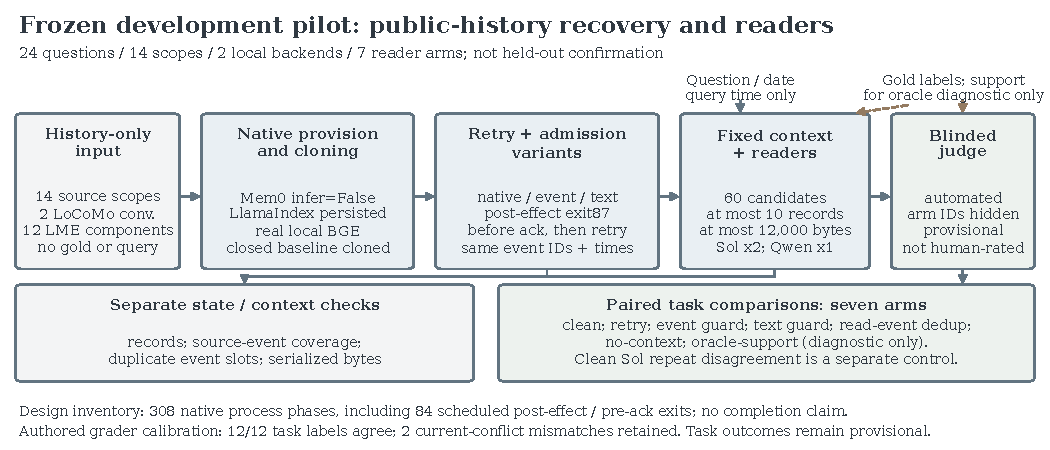
\includegraphics[width=\linewidth]{figures/fig_frozen_development_pilot_design.pdf}
\caption{Frozen development protocol and information boundaries. The figure separates ingestion input, query date, annotated support, and automated judging; it identifies the local raw-document paths and the failed auxiliary calibration.}
\label{fig:design}
\end{figure}

\section{Results}
\subsection{Physical multiplicity and returned evidence}
All original records remained present after replay, but the number of distinct returned source events fell on many queries. Across the 24 questions, event counts decreased on 20/24 Mem0 contexts and 16/24 LlamaIndex contexts. Annotated positive-support coverage decreased on 1/23 available Mem0 cases and 4/23 LlamaIndex cases; one case per backend had no applicable support annotation. These annotation counts are not exhaustive semantic judgments and the question scopes overlap. The complete per-question matrix, including unchanged and null cells, is shown in Figure~\ref{fig:contexts}.

The automated task grader flags seven backend/reader/question loss combinations across four unique questions and eleven dependent repeat transitions; it flags no gains under the audited task label. Event dedup recovers every flagged task label. Five LlamaIndex combinations recover the exact clean prompt and alias its response; two Mem0 combinations yield distinct prompts and separately archived responses. These are descriptive finite-pilot counts. Because of the failed current-conflict calibration and same-family judge, they are not evidence of a measured stale-memory rate or a validated semantic repair.

\begin{figure}[t]
\centering
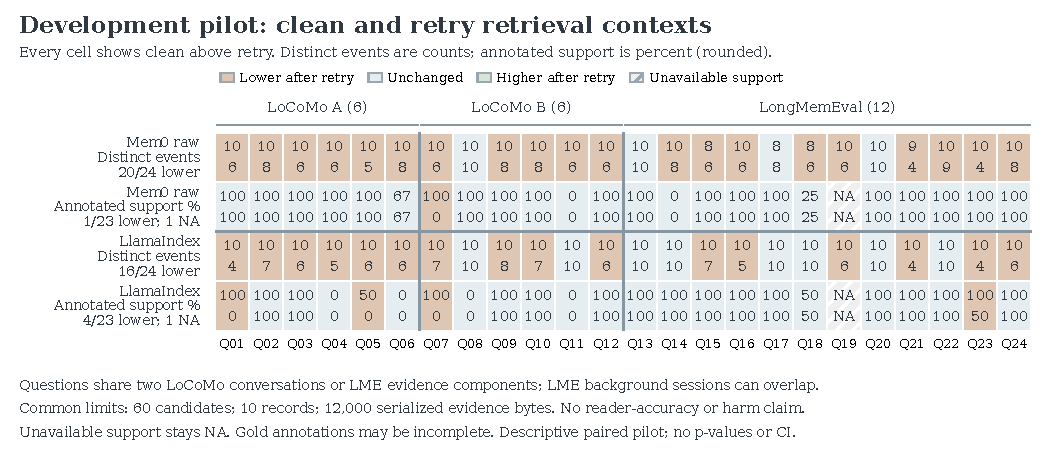
\includegraphics[width=\linewidth]{figures/fig_pilot_context_structure.pdf}
\caption{Per-question event-count and annotated positive-support changes under clean and replayed contexts for all 24 development questions and both storage paths. Unchanged cells and unavailable annotations are retained. Each row is a question from shared conversations, not an independent population draw.}
\label{fig:contexts}
\end{figure}

\subsection{A trace-level answer failure}
Question \texttt{45dc21b6} asks how many of Emma's recipes the user had tried. In the public history, one dated statement says two on May 29 and a later statement says three on May 30; the benchmark reference is three. In the clean LlamaIndex context, both statements are selected. After replay, the older statement has three physical instances and occupies ranks 1--3; the newer statement remains unchanged in storage and appears at native candidate rank 11, beyond the ten-record context. The returned context contains six duplicate event slots and only four distinct events. Both GPT-6.1-Sol repeats and the Qwen3 reader answer two. Their clean archived answers say three.

The changed answer follows the changed evidence: the two-count source event is present in the replay context; the later three-count source event is not. Selecting distinct source occurrences from the same native candidate sequence restores the clean ten-event context. The resulting complete prompt is byte-identical to the clean prompt, so the protocol reuses the archived clean answer. This supports a claim about input/context restoration. It is not a new generation-level demonstration that a model repairs itself after deduplication. The case was inspected after the pilot and does not add a sample.

\subsection{Deduplication and residual ranking drift}
Ordinary event deduplication and corpus-statistics restoration are different interventions. For LlamaIndex, deduplication restores all 24 contexts in this finite pilot. For Mem0, 16/24 contexts still have a different selected event set at the common returned-candidate budget after event deduplication, even though task labels recover. This does not establish a residual task loss.

A frozen post-hoc probe asks why. On copies of clean and replayed Mem0 stores, 96 native explain queries cover clean/replayed copies of the same 24 questions at returned limits of 60 and 10,000. The native path combines semantic similarity, normalized BM25, and entity contributions additively; it is not reciprocal-rank fusion. The probe finds that semantic and entity contributions for original points remain stable, while normalized BM25 and final scores change for all 24 queries. With full candidate pools, event dedup still leaves 10/24 selected event sets and 17/24 event orders different. Each changed event set contains a strict lost/gained score-order reversal, not solely a tie-breaking change. This is a post-hoc mechanistic probe on reused queries, not additional task evaluation.

The tested Qdrant implementation computes sparse-term IDF from physical point counts, using $\operatorname{IDF}(t)=\log(1+(N-df(t)+0.5)/(df(t)+0.5))$. Repeated physical copies can therefore alter the sparse score contribution while the logical source-event set is unchanged. In a counterfactual, duplicate points remain searchable but the native IDF corpus parameter is restricted to the original clean physical IDs. The clean full-pool event orders and contexts return for all 24 queries; all five score components match clean values within $10^{-12}$ across 12,320 original-point comparisons. This intervention supplies known clean IDs and is an oracle mechanism control, not an oracle-free policy. The independent ranking audit verifies 52,740 rows, native payload membership, score equations, and selected order. Raw sparse-dot-product reconstruction was not retained, so the component drift is verified through the recorded native scores and counterfactual, not by recomputing every vector dot product from the archive.

\begin{table}[t]
\centering
\small
\begin{tabularx}{\linewidth}{@{}l X@{}}
\toprule
Observation & Audited result and interpretation \\
\midrule
Native replay & 84 authored post-effect cuts; original records/payload fingerprints preserved. Controlled schedule, not natural incidence. \\
Context event count & Decreased in 20/24 Mem0 and 16/24 LlamaIndex replay contexts; finite, overlapping development questions. \\
Task labels & Seven loss combinations, four questions, eleven dependent repeats; no gains; event dedup restores all flagged labels. Automated and exploratory. \\
Recipe witness & Latest count remains stored, moves rank 5 to 11, leaves top-10 context; both readers change 3 to 2. One inspected case. \\
Full-pool Mem0 probe & After event dedup, 10/24 event sets and 17/24 orders differ; post-hoc reranking analysis, not new questions. \\
Fixed-IDF counterfactual & All 24 contexts restored with clean physical IDs defining IDF corpus; oracle diagnostic, not deployment method. \\
\bottomrule
\end{tabularx}
\caption{Primary finite-study findings and limits. Repeated prompts, grading aliases, and mechanistic probes do not increase the 24-question development set.}
\label{tab:results}
\end{table}

\begin{table}[t]
\centering
\small
\begin{tabular}{@{}lllc rr r@{}}
\toprule
Dataset & Backend & Reader & $n$ questions & Clean & Replay & Event dedup \\
\midrule
LoCoMo & Mem0 raw & Sol & 12 & 0.833 & 0.750 & 0.833 \\
LongMemEval-S & Mem0 raw & Sol & 12 & 0.917 & 0.917 & 0.917 \\
LoCoMo & Mem0 raw & Qwen3 & 12 & 0.667 & 0.667 & 0.667 \\
LongMemEval-S & Mem0 raw & Qwen3 & 12 & 0.583 & 0.500 & 0.583 \\
LoCoMo & LlamaIndex & Sol & 12 & 0.583 & 0.417 & 0.583 \\
LongMemEval-S & LlamaIndex & Sol & 12 & 0.917 & 0.833 & 0.917 \\
LoCoMo & LlamaIndex & Qwen3 & 12 & 0.500 & 0.417 & 0.500 \\
LongMemEval-S & LlamaIndex & Qwen3 & 12 & 0.583 & 0.500 & 0.583 \\
\bottomrule
\end{tabular}
\caption{Exploratory automated task-label means for the three principal answer conditions. Sol repeats are averaged within question; each row has 12 questions, with shared histories and prompt aliases. These values are descriptive, not independent-sample estimates or a validated comparison of systems.}
\label{tab:taskmeans}
\end{table}

\section{Discussion}
The concrete finding is a separation of invariants. Physical preservation did not imply that the retriever exposed the same evidence. Event-level deduplication was sufficient to restore all task labels flagged as losses in this finite pilot, while a separate controlled intervention was needed to reproduce all tested Mem0 contexts after the full-pool probe. The two results are compatible: a task can be answered correctly from more than one context, and a changed context need not change the task label.

The fixed-IDF counterfactual identifies one local mechanism, rather than a general cure. Because Qdrant's corpus statistics count physical points, replay changes the BM25 component even when original vectors and logical events are preserved. Restricting those statistics to the original clean population restores the observed order in this pinned setup. This is consistent with known duplicate sensitivity in classical IR and recent redundancy research \citep{frieder2003scalable,robertson2009probabilistic,schelpe2026byte,jain2026cuer}. We therefore describe the result as application-specific causal localization and a testable conformance witness. We do not claim a new IDF formula, deduplication algorithm, ranking theorem, or first discovery of duplicate-induced ranking changes.

An operational implication for system testing is to preserve identifiers for source occurrences separately from physical records, and to evaluate at least three outputs after replay: physical state, selected source-event sequence, and task result. A test that checks only whether a write exists can miss evidence drift; a test that checks only task accuracy can miss changed ranking that happens not to matter for that query. This recommendation is an inference from the measurements, not a validated production intervention.

The direction of aggregate metrics also matters. Token F1 can improve while task labels remain unchanged; event counts and annotated support can decline without a validated semantic error; and deduplication can recover task labels while contexts remain different. Reporting a single score would erase these distinctions. In particular, the grader's current-conflict calibration did not meet its declared threshold. We retain all automated labels but use them only descriptively.

\section{Limitations and Validity}
\paragraph{Sample and external validity.} This is one public-data development selection of 24 questions from 14 history scopes, including only two LoCoMo conversations. Histories and backgrounds can overlap, and no random or held-out selection was used. The 96-query and 120-query diagnostics reuse these same questions. Findings do not estimate natural failure incidence, prevalence across agent deployments, or performance across a population of memory systems.

\paragraph{System scope.} Mem0 was tested with inference disabled and local Qdrant; LlamaIndex stored raw documents in a local vector path. These settings omit hosted services, extraction pipelines, model-based memory mutation, production concurrency, and other indexes. Both local paths share public embedding/provider components. The authored cut is after a native effect, and does not test transport-level loss or mid-commit failure. The sequential admission controls do not prove concurrent uniqueness; content-based deduplication may also suppress legitimate repeated observations if occurrence identity is lost.

\paragraph{Reader and judge validity.} Sol request configuration was not fully attested, and its judge is same-family as one reader. The independent Qwen3 responses add a different local model family but not independent human labels. The auxiliary calibration passed task labels but failed current-conflict labels (10/12), precluding a definitive semantic conflict claim. One invalid citation was retained, and five apparent recoveries are exact-prompt aliases rather than fresh generations. No model or system superiority is tested.

\paragraph{Metrics and auditability.} Annotated positive support is incomplete by design and is not exhaustive evidence coverage. Token metrics are lexical proxies. A Unicode scorer discrepancy was corrected in a separate helper; measured official-metric differences were not material in the 504 audited LoCoMo aliases, but that check does not validate every benchmark scorer or answer. The native score audit does not preserve raw sparse dot products for independent vector-level reconstruction. All these constraints are retained in the artifacts.

\paragraph{Novelty and venue readiness.} Duplicate documents' effects on IDF and ranking are explicit prior art, and contemporary RAG work evaluates redundancy, evidence quality, and deduplication. This manuscript's candidate addition is the linked native delivery-replay, physical-state, evidence-selection, and reader trace, plus a local counterfactual that isolates statistics in one configuration. Whether this constitutes a sufficiently general systems contribution remains open. Before submission to a selective journal, the study needs independent replication, held-out histories, broader storage/index implementations, human-adjudicated outcomes with a successful calibration, and review by domain experts. We make no claim that the current evidence meets Q1 journal standards.

\section{Conclusion}
In this controlled development study, repeated native delivery preserved the original stored memories while changing evidence selected for later questions. A dated recipe-count trace shows how an unchanged later fact can move outside a finite context and how two readers can then report an older count. Event deduplication recovered the finite pilot's flagged task labels but did not universally restore retrieval order. In a post-hoc local Mem0/Qdrant diagnostic, corpus-statistics control restored all 24 full-pool contexts, consistent with established duplicate-sensitive IDF behavior. These results provide an inspectable conformance case and a concrete next research direction, not a breakthrough claim, general reliability rate, or journal acceptance case.

\section*{Artifacts, authorship, and assistance}
The protocols, native stores, reader inputs and responses, grading packets, audit scripts, and reports are versioned in the public repository branch \href{https://github.com/aditya-genies/beyond-recall/tree/codex/benchmark-impact}{\texttt{codex/benchmark-impact}}. The release archive is intended to permit review of frozen native artifacts without employer data or credentials. The earlier v0.3.0 working paper is a separate historical artifact; its results are not pooled with this study. PaperOrchestra was used to structure research inputs and the manuscript workflow; AI tools assisted with implementation and drafting. The author is solely responsible for the claims, data handling, and final text. Automated audits are not peer review. No funding or institutional endorsement is claimed.

\bibliographystyle{unsrtnat}
{\small\bibliography{refs}}
\end{document}
